\documentclass[fleqn, 12pt]{extarticle}
\usepackage{textbook}

\begin{document}
\selectlanguage{russian}

\title{\textbf{Организация Станций Страховки}\\
\large{Краткое Справочное Пособие для Новичков}}
\author{\textsc{Юлия Беляева}\\\textit{а/к Политехник}}
\date{2014}

\maketitle

\begin{abstract}
	Данное справочное пособие является дополнением к лекциям и тренировкам, проводимым для новичков альпклуба <<Политехник>>. Оно описывает лишь некоторые принципы и техники организации станций,
	оставляя за рамками многие вещи, которые разбираются на тренировках и практических занятиях. Использование данного материала для самостоятельного изучения темы с нуля без инструктора не
	рекомендуется.
\end{abstract}

\section{Качества хорошей станции}
    Станции оценивают по следующим качествам:
    \begin{itemize}
        \item \textbf{Надёжность.} Станция должна выдерживать всевозможные нагрузки, которые могут на неё прийтись: статические нагрузки, создаваемые висящими на станции людьми
                и снаряжением, и динамические нагрузки, вызванные срывами. Наиболее опасен срыв лидера сразу после станции до постановки первой точки (срыв с фактором близким к двум),
                так как нагрузка на станцию в этот момент наибольшая. Надёжность станции прежде всего зависит от надёжности точек, на которых она основана. 
                Из плохо поставленных точек невозможно получить надёжную станцию даже при помощи самых хитроумных техник.
        \item \textbf{Дублирование} означает, прежде всего, использование нескольких точек для организации станции, чтобы предотвратить разрушение её в случае отказа одной из точек. 
                Кроме того, часто дублируют петли, в особенности, если есть опасность их попадания на острую скальную кромку. Также понятие дублирования включает в себя использование 
                для станции нескольких разных элементов рельефа, например, вместо того чтобы располагать все точки в одной и той же щели.
        \item \textbf{Равномерное распределение нагрузки} означает, что вся нагрузка, действующая на станцию, не приходится целиком на одну из точек, а распределяется между ними. 
                Тем самым уменьшается риск отказа точек. Важно помнить, что нагрузка действующая на станцию не обязательно направлена вертикально вниз, она может быть направлена как 
                и под небольшим углом к вертикали, так и сильно в сторону. Кроме того при срыве лидера рывок на станцию может быть направлен вверх. Возможные направления рывка 
                необходимо учитывать при организации станции.
        \item \textbf{Отсутствие проседания} означает, что при отказе одной из точек станция не должна сильно проседать, создавая динамическую нагрузку на оставшиеся точки.
    \end{itemize}
    
    Важно понимать, что:
    \begin{itemize}
        \item эти четыре качества не являются исчерпывающими, это просто хорошая практика организации станций;
        \item невозможно удовлетворить этим качествам на сто процентов, нужно удовлетворить им достаточно хорошо для данной ситуации, затратив не слишком много времени и снаряжения; 
              при этом станция должна оставаться как можно более простой;
        \item качества <<равномерное распределение нагрузки>> и <<отсутствие проседания>> конфликтуют между собой, в зависимости от ситуации отдаётся приоритет одному из них.
    \end{itemize}

\section{Станции на одной точке}
    Станции на одной точке организуют на естественных элементах рельефа: деревьях, больших валунах, скальных выступах, отколах. Важно убедиться в абсолютной надёжности единственной точки. 
    Шлямбура, а также закладки, крючья, ледобуры и т.п. не считаются достаточно надёжными для использования в качестве единственной точки станции.
    \begin{figure}[h]
        \centering
        \begin{minipage}[t]{0.45\textwidth}
            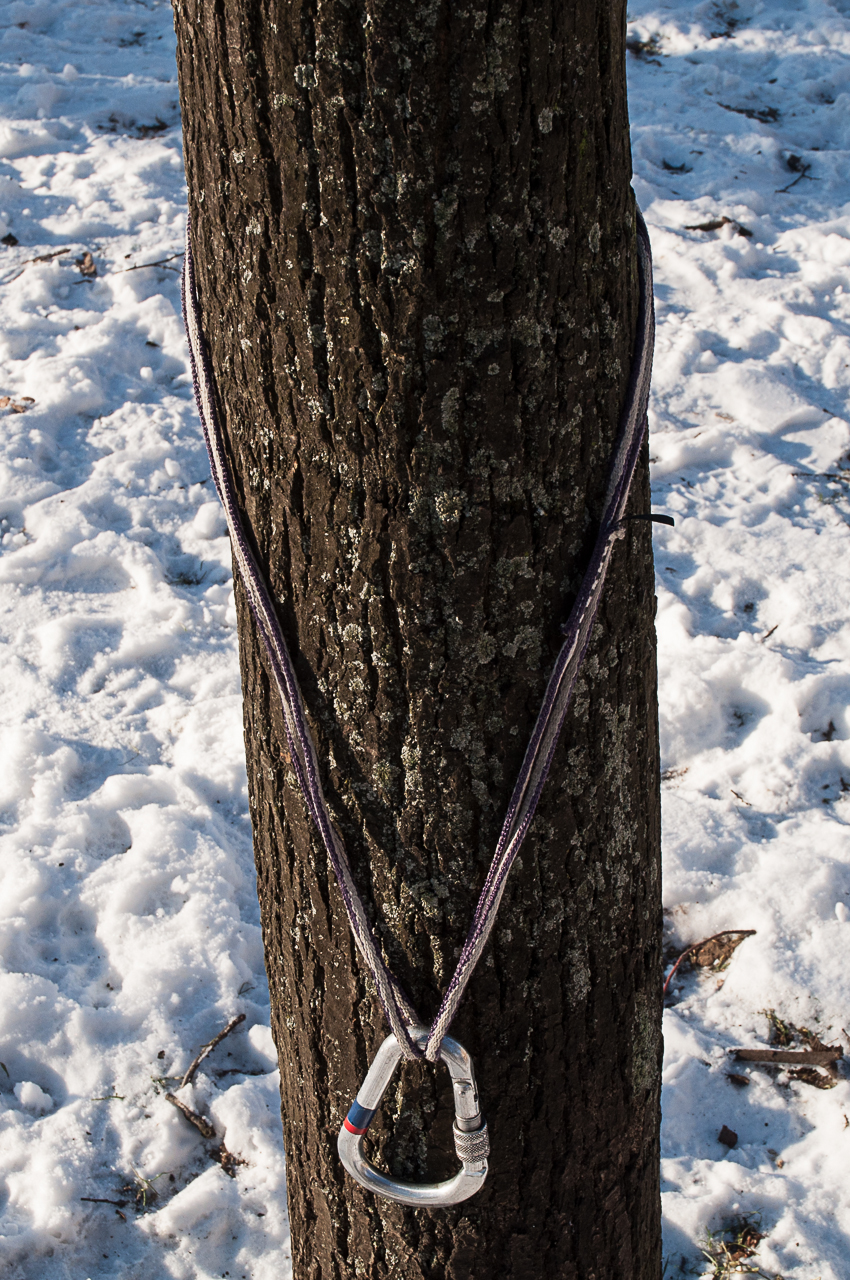
\includegraphics[width=\textwidth]{tree1}
            \captionof{figure}{Простейший вариант станции на дереве.}\label{fig:tree1}
        \end{minipage}\hspace{0.05\textwidth}
        \begin{minipage}[t]{0.45\textwidth}
            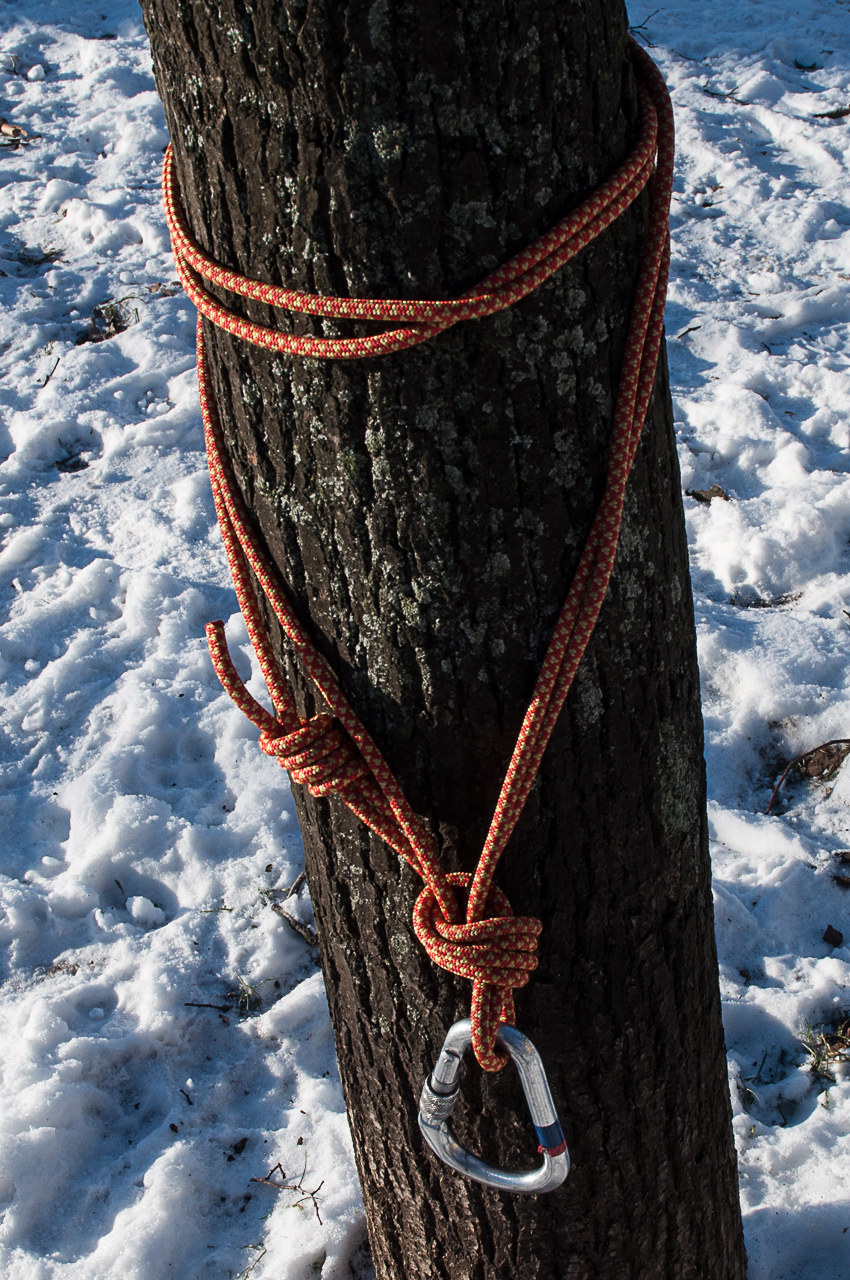
\includegraphics[width=\textwidth]{tree2}
            \captionof{figure}{Улучшенный вариант станции с центральным узлом и дополнительным оборотом вокруг ствола дерева.}\label{fig:tree2}
        \end{minipage}
    \end{figure}

   	\newpageПри организации станции дереве важно проверить что:
    \begin{itemize}
        \item дерево живое, не сухое и неповреждённое;
        \item оно достаточно большое;
        \item оно хорошо сидит в почве (для этого дерево можно потрясти).
    \end{itemize}
    
	Простейшая станция на дереве организуется оборачиванием петли вокруг ствола (рис.~\ref{fig:tree1}). В два конца петли вставляется карабин, который играет роль центрального пункта станции.
    Карабин в центральном пункте также называют мастер-карабином или станционным карабином. Важно чтобы угол между двумя концами петли, в которые продет станционный карабин, был острым
    (см. разд.~\ref{sec:multipoint.anchors}). Для того чтобы зафиксировать правильное положение станционного карабина и исключить возможность его нагрузки в трёх направлениях 
    при достаточной длине петли на ней завязывают узел (восьмёрка или проводник). Этот узел также обеспечивает дублирование в петле. Кроме того, сама по себе  петля узла уже может играть 
	роль центрального пункта, что делает использование станции более удобным. Для того чтобы зафиксировать положение станции на дереве можно сделать дополнительный оборот петли
    вокруг ствола (рис.~\ref{fig:tree2}),
	если это позволяет длина петли. Желательно избегать использования узла удавка для этих целей, так как он сильно ослабляет стропу.
    Не рекомендуется делать станцию высоко на стволе дерева из-за образующегоcя рычага.
    
    Особенности использовании элементов скального рельефа в качестве единственной точки станции:
    \begin{itemize}
        \item используемый элемент рельефа должен быть большим;
        \item валуны держатся на месте не только за счёт своего веса, но и за счёт расположения, важно проверить что используемый валун не сможет сдвинуться с места;
        \item выступы и отколы должны быть хорошо соединены с основной скалой;
        \item необходимо подвигать, покачать используемый выступ, откол или камень, он должен быть абсолютно неподвижен;
        \item нужно постучать по скале молотком и убедиться что она издаёт звонкий звук;
        \item скалы не должны иметь острые края, которые могли бы перерезать петлю/репшнур;
        \item форма выступа не должна позволять петле с него соскочить.
    \end{itemize}
    
    Полезно придерживаться этих же рекомендаций при использовании элементов рельефа в качестве промежуточных точек страховки.
    \begin{figure}[h]
        \centering
        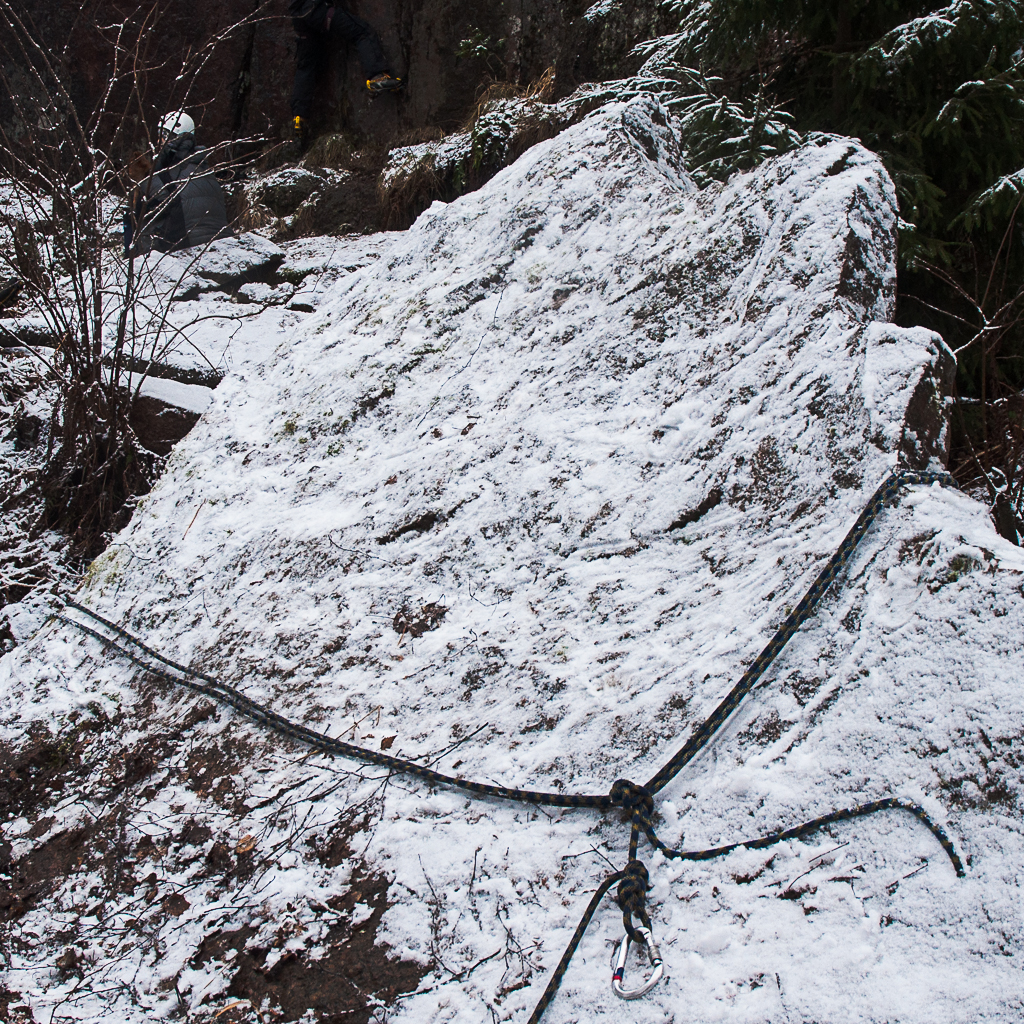
\includegraphics[width=0.45\textwidth]{bowline}
        \caption{Станция на выступе из основной верёвки, завязанной двойным булинём.}\label{fig:bowline}
    \end{figure}
    
    Станции на рельефе организуются оборачиванием или набрасыванием петли на элемент рельефа аналогично станциям на дереве. Кроме петель из стропы или репшнура можно использовать
    связочную верёвку, завязав на конце двойной булинь (рис.~\ref{fig:bowline}). Также для организации станций можно использовать песочные часы -- сквозные отверстия в скале --
    или пробки -- заклинившие в каминах или расщелинах обломки скалы, продевая через них петлю или репшнур.

\section{Станции на нескольких точках}\label{sec:multipoint.anchors}
    Существует множество способов блокировки (объединения) нескольких точек в станцию. В наиболее распространённых методах точки блокируются друг с другом
    так, что центральный пункт станции соединён с каждой точкой отдельной ветвью из репшнура или стропы. При этом нагрузка на центральный пункт распределяется между ветвями.
    Распределение сил в станции зависит от направления приложенной силы и угла между ветвями станции
    (табл.~\ref{tab:angle}). Для некоторых способов блокировки (например, для станции с фиксированным центральным узлом, разд.~\ref{sec:cordelette}) оно так же зависит от разницы длин ветвей.
    \begin{table}[h]
        \centering
        \begin{tabular}{|c|c|}
            \hline
            \multirow{2}{*}{угол между ветвями станции} & процент от общей нагрузки \\ & приходящийся на каждую точку \\
            \hline
            $30^o$ & $52\%$ \\
            $45^o$ & $54\%$ \\
            $60^o$ & $58\%$ \\
            $90^o$ & $71\%$ \\
            $120^o$ & $100\%$ \\
            $150^o$ & $193\%$ \\
            $170^o$ & $574\%$ \\
            \hline
        \end{tabular}
        \caption{Распределение нагрузки между двумя точками станции в зависимости от угла между её ветвями.}\label{tab:angle}
    \end{table}
    
    Изменение направления нагрузки по-разному влияет на её распределение между точками в зависимости от выбранной схемы блокировки. Схемы которые при изменении направления
    действующей силы перестраиваются и продолжают грузить точки с одинаковой силой, называются схемами с динамическим (или автоматическим) распределением, а процесс перестройки 
    называется компенсацией. Минусом компенсации является наличие некоторого количества слабины в системе, из-за которой при отказе одной из точек происходит проседание станции. 
    Схемы с жёсткой блокировкой точек, не допускающей перестройку, называются схемами со статическим распределением нагрузки. Минусом таких схем, кроме отсутствия компенсации,
    является то что при разной длине ветвей станции при рывке короткая ветвь будет нагружена больше, чем длинная.

\subsection{Компенсационная петля и её варианты}
    Компенсационная петля является схемой с динамическим распределением нагрузки.
    
    \subsubsection{Компенсационная петля на двух точках}
    При организации станции с использованием компенсационной петли (рис.~\ref{fig:slidx2}) важно сделать правильный перекрут в одной из ветвей петли (рис.~\ref{fig:slidx2_details}).
    Благодаря этому станция не развалится при отказе одной из точек. В такой схеме станционный карабин свободно перемещается по петле, что позволяет станции хорошо распределять
    нагрузки между точками в широком диапазоне направлений.
    Способность карабина перемещаться зависит от трения в петле. Поэтому компенсационная петля хорошо работает с тонкими дайнимовыми стропами или репшнуром и хуже
    с толстыми нейлоновыми стропами. Сшивка петли (или узел на репшнуре) не должна мешать станционному карабину скользить по петле, лучше их располагать ближе к одной из точек.
    На станции с разными длинами плеч сшивка (узел) должна находиться на коротком плече, чтобы не попасть в станционный карабин при возможном перевороте станции.
    \begin{figure}
        \centering
        \begin{minipage}[t]{0.45\textwidth}
            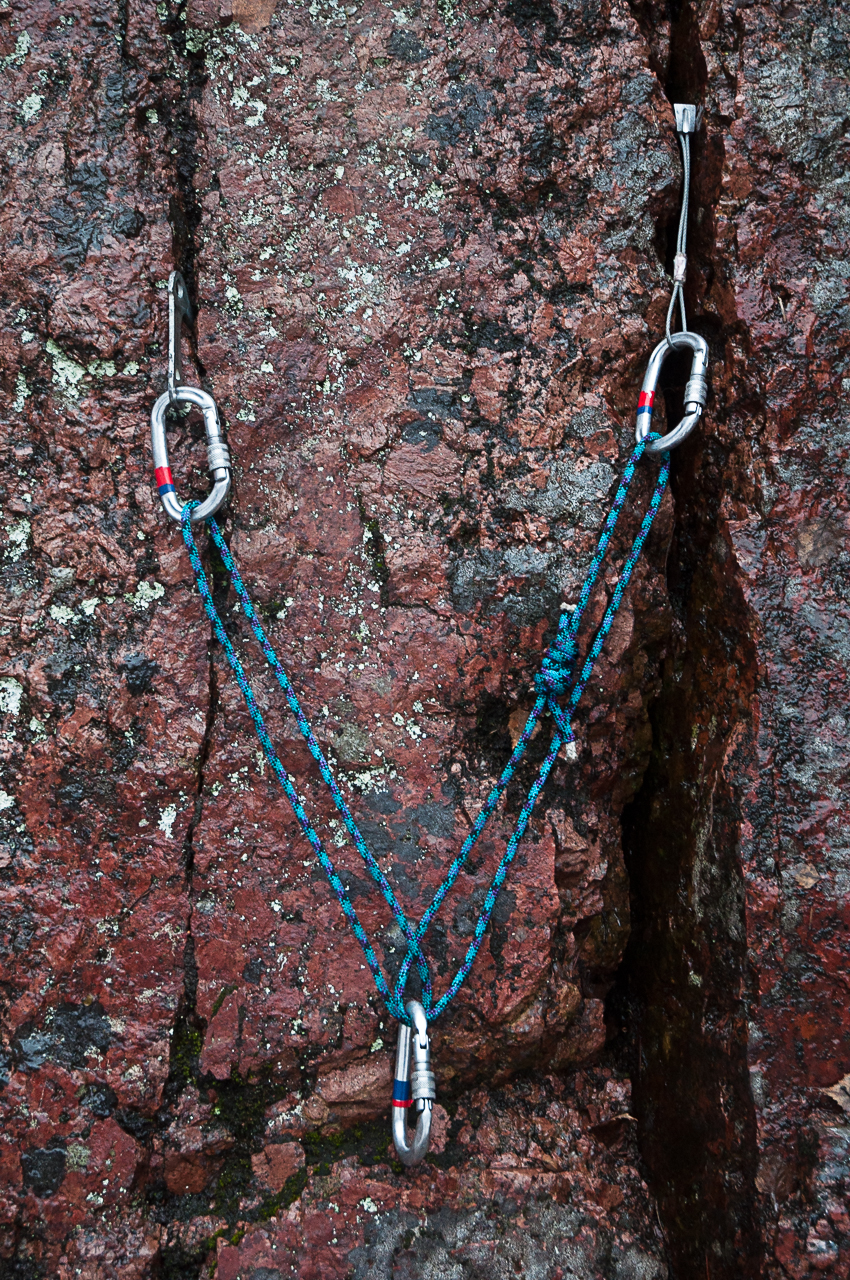
\includegraphics[width=\textwidth]{slidx2}
            \captionof{figure}{Классическая компенсационная петля на двух точках.}\label{fig:slidx2}
        \end{minipage}\hspace{0.05\textwidth}
        \begin{minipage}[t]{0.45\textwidth}
            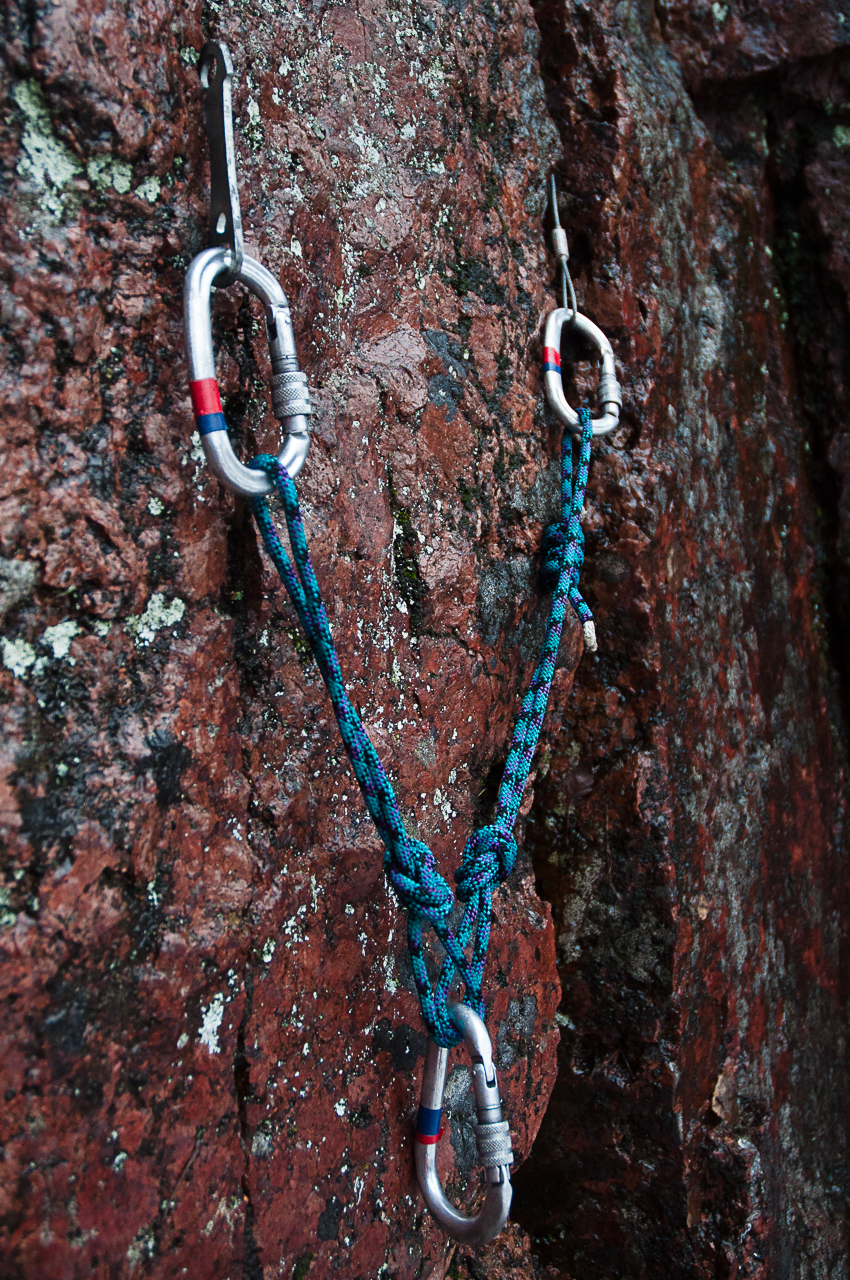
\includegraphics[width=\textwidth]{slidx2_knots}
            \captionof{figure}{Компенсационная петля с узлами-ограничителями на двух точках.}\label{fig:slidx2_knots}
        \end{minipage}
    \end{figure}
    
	Главным недостатком компенсационной петли является сильное проседание станции при отказе одной из точек, которое приводит к большой динамической нагрузке на оставшуюся точку.
    Поэтому такая станция может быть опасной на потенциально слабых точках. Кроме того, в данной схеме отсутствует дублирование в петле. Это значит, что при разрыве петли, например
    при попадании на острую скальную кромку, станция полностью разрушается.
    
    Завязывание узлов-ограничителей (проводник или восьмёрка, рис.~\ref{fig:slidx2_knots}) позволяет сократить возможное проседание станции до приемлемого (за счёт уменьшения степени компенсации)
    и обеспечивает дублирование петли.
    
    \begin{figure}
        \centering
        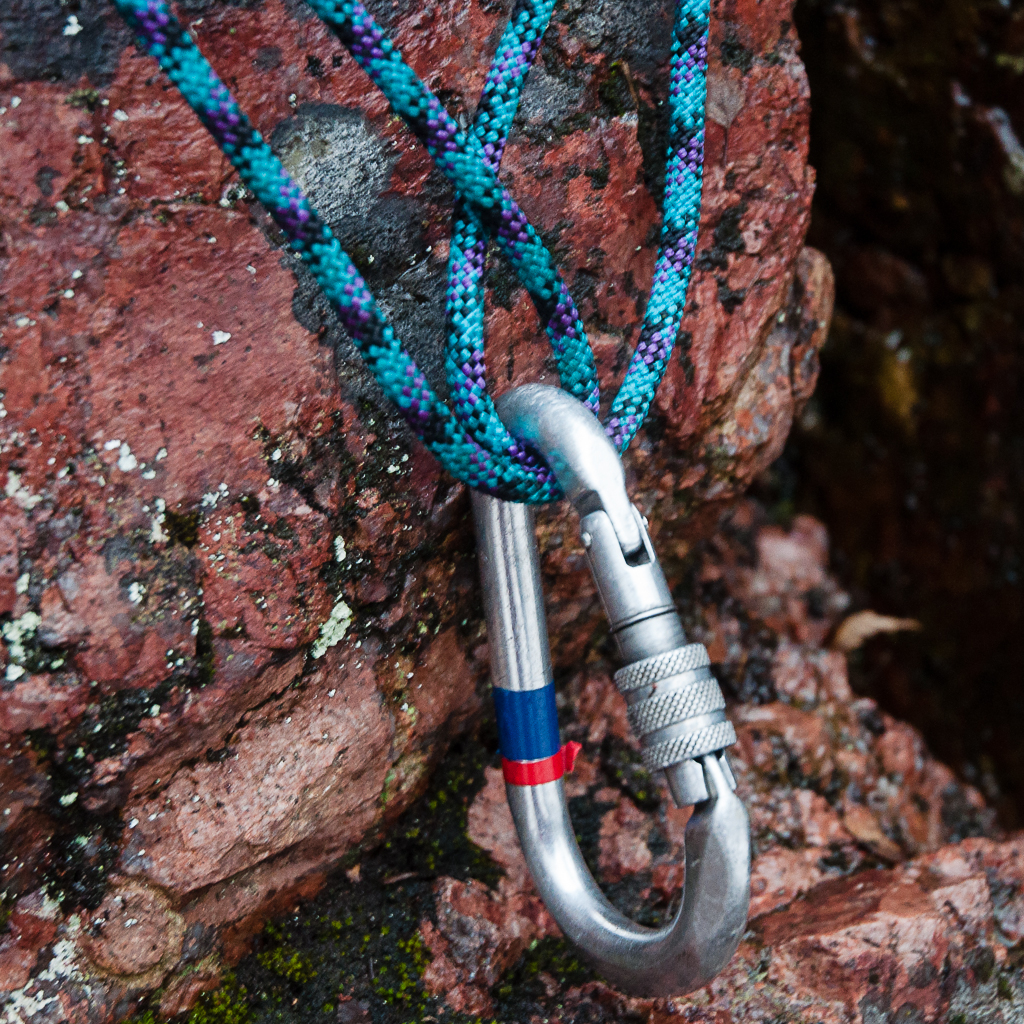
\includegraphics[width=0.45\textwidth]{slidx2_details}
        \caption{Центральный пункт в классической компенсационной петле крупным планом.}\label{fig:slidx2_details}
    \end{figure}
    
    \subsubsection{Компенсационная петля на трёх точках}
    \begin{figure}[h]
        \centering
        \begin{minipage}[t]{0.45\textwidth}
            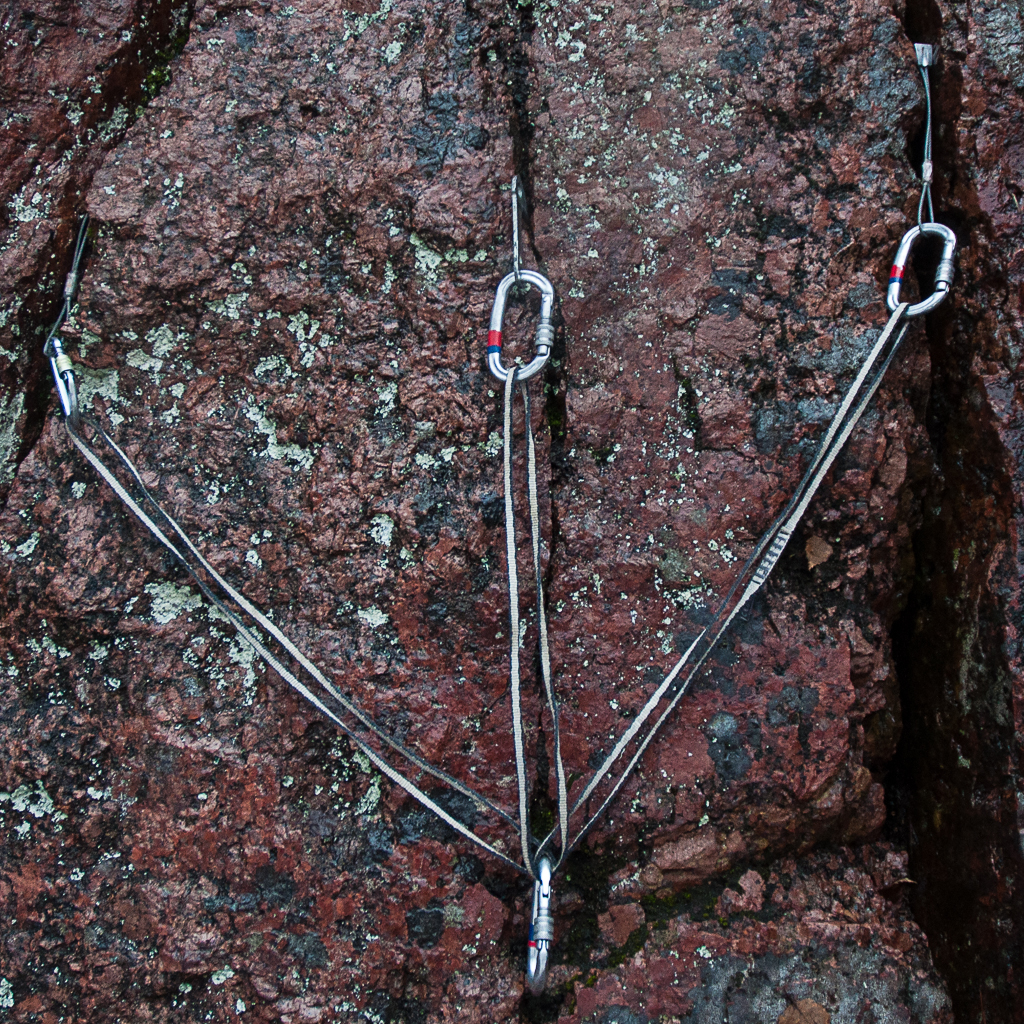
\includegraphics[width=\textwidth]{slidx3}
            \captionof{figure}{Классическая компенсационная петля на трёх точках.}\label{fig:slidx3}
        \end{minipage}\hspace{0.05\textwidth}
        \begin{minipage}[t]{0.45\textwidth}
            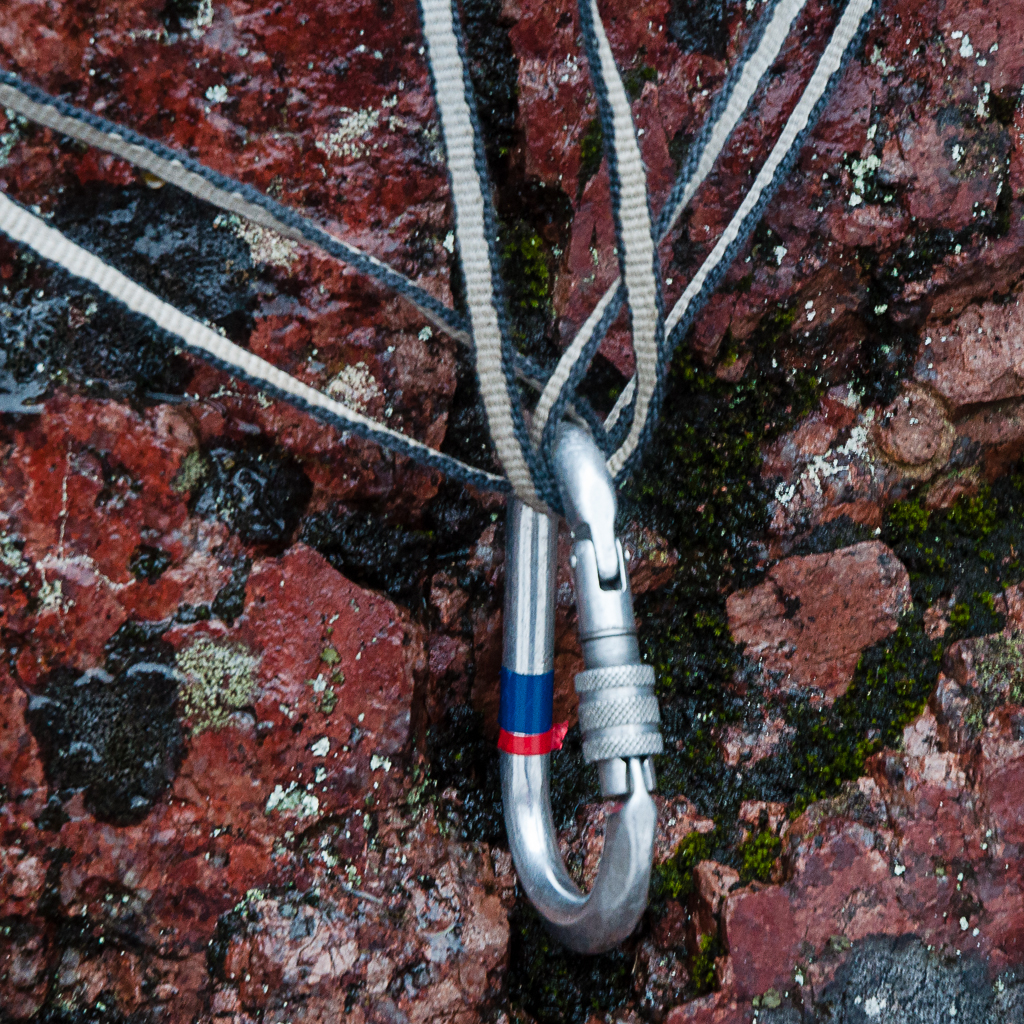
\includegraphics[width=\textwidth]{slidx3_details}
            \captionof{figure}{Центральный пункт классической компенсационной петли на трёх точках крупным планом.}\label{fig:slidx3_details}
        \end{minipage} 
    \end{figure}
    \newpageКлассическая компенсационная петля на трёх точках (рис.~\ref{fig:slidx3}) получается аналогично компенсационной петле на двух точках. На петле между соседними точками делаются перекруты
    (рис.~\ref{fig:slidx3_details}),
    которые объединяются друг с другом и третьей ветвью петли. Данная схема реагирует на изменение направления нагрузки гораздо хуже, чем компенсационная петля на двух точках
    из-за большего трения в мастер-карабине. На толстых нейлоновых стропах станцию может заклинить, поэтому не рекомендуется использование таких строп для этой схемы.
    Завязывание узлов-ограничителей возможно только на двух из трёх ветвей станции (если завязать узел на третьей ветви то теряется компенсация). Это не позволяет в полной мере
    ограничить проседание станции.
    
    Из-за вышеперечисленных недостатков не рекомендуется использовать классическую компенсационную петлю на трёх точках. Лучше использовать станцию с фиксированным центральным узлом
    (разд.~\ref{sec:cordelette}) или компенсационную петлю на трёх точках со стременами.
    \begin{figure}[h]
        \centering
        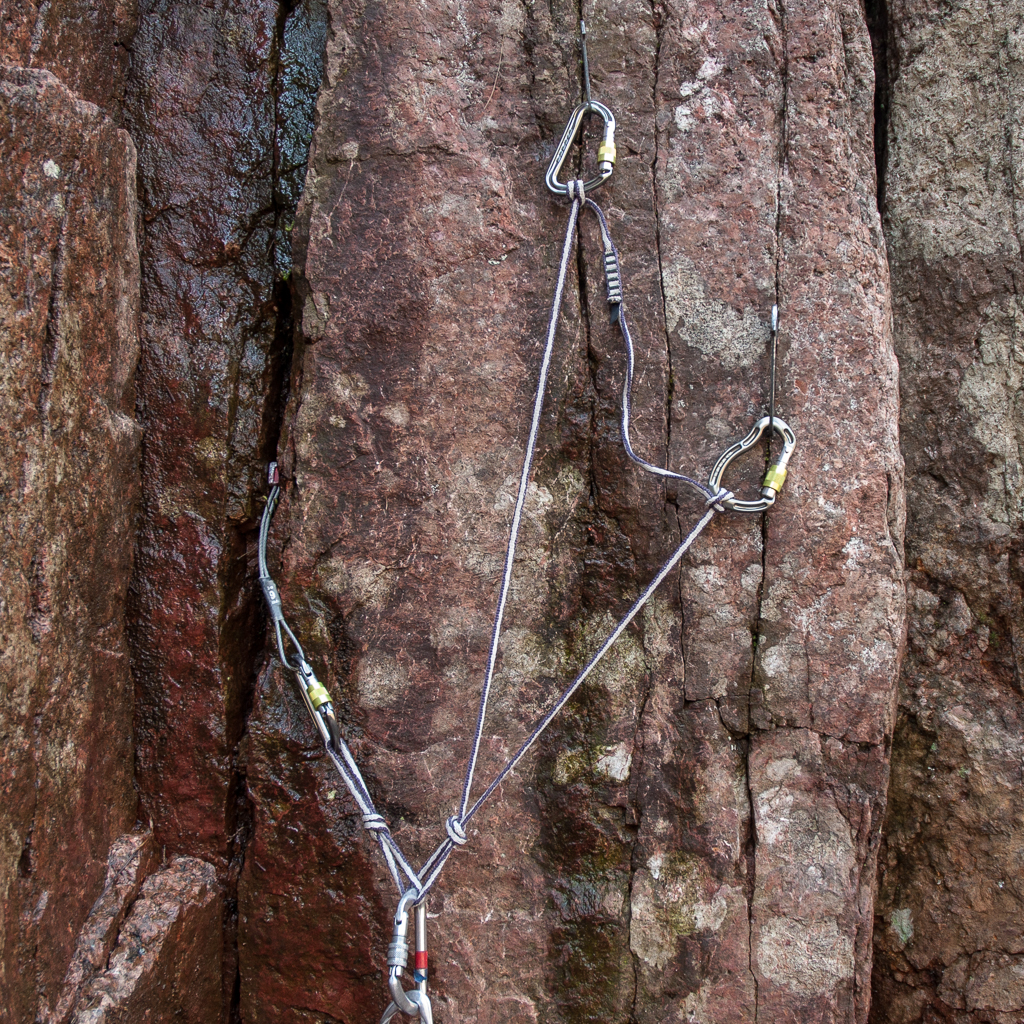
\includegraphics[width=0.45\textwidth]{slidx3_clove}
        \caption{Компенсационная петля на трёх точках со стременами.}\label{fig:slidx3_clove}
    \end{figure}
    
    Компенсационная петля на трёх точках со стременами (рис.~\ref{fig:slidx3_clove}) организуется так же как и компенсационная петля на двух точках с ограничителями,
    при этом на одной ветви петли завязываются
    стремена и вешаются на две соседние точки таким образом, чтобы стропа между ними была не натянута. Такая станция компенсирует изменение направления нагрузки так же хорошо,
    как и компенсационная петля на двух точках: на каждую из ветвей станции будет приходиться приблизительно половина нагрузки. Однако в ветви со стременами нагрузка уже не будет
    распределяться равномерно, так как точки со стременами соединены фактически фиксированной связью. Из-за этого важным при организации такой станции будет подбор правильного
    положения стремян на точках.

\subsection{Станция с фиксированным центральным узлом}\label{sec:cordelette}
    Станция с фиксированным центральным узлом является схемой со статическим распределением нагрузки.

    \subsubsection{Станция с фиксированным центральным узлом на двух и трёх точках}
    \begin{figure}[h]
        \centering
        \begin{minipage}[t]{0.45\textwidth}
            \centering
            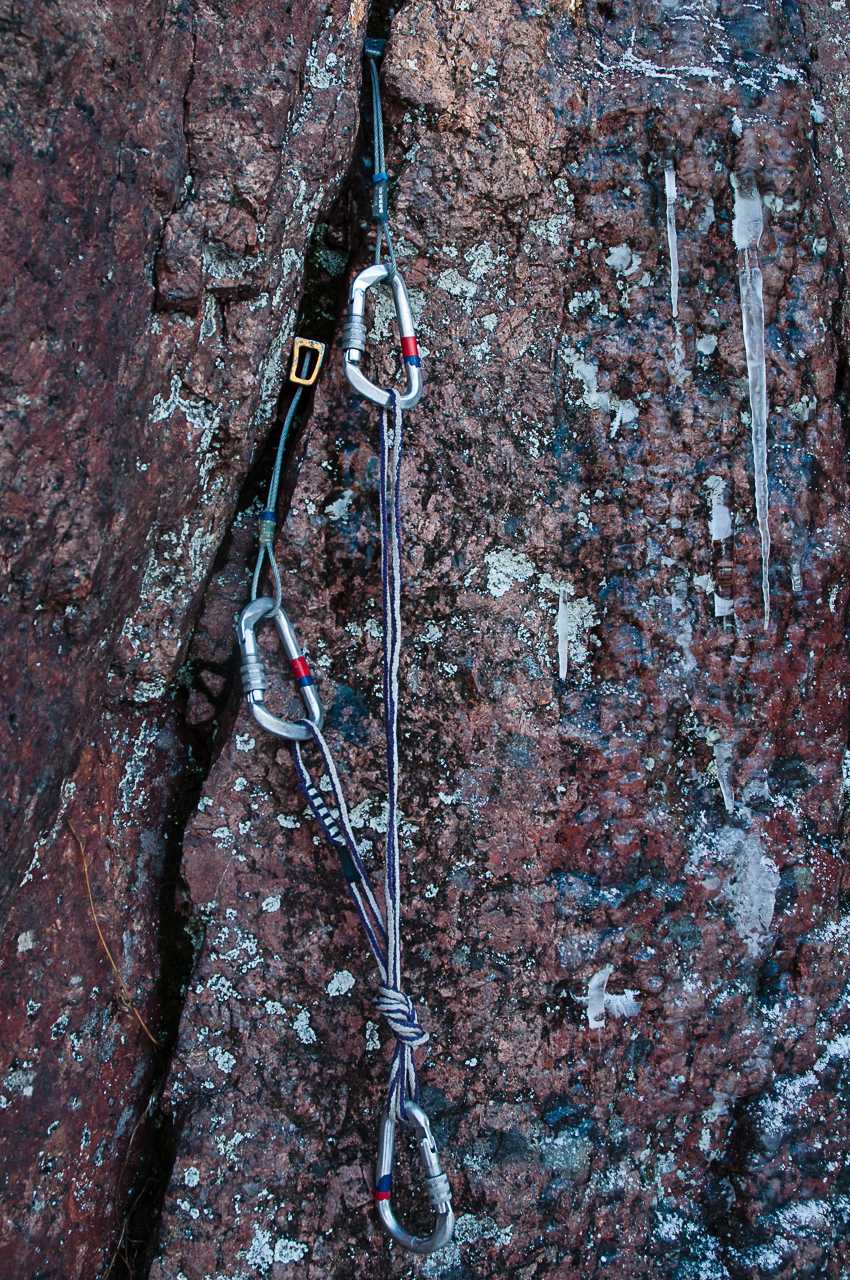
\includegraphics[width=\textwidth]{cordelette2}
            \captionof{figure}{Станция с фиксированным центральным узлом на двух точках.}\label{fig:cordelette2}
        \end{minipage}\hspace{0.05\textwidth} 
        \begin{minipage}[t]{0.45\textwidth}
            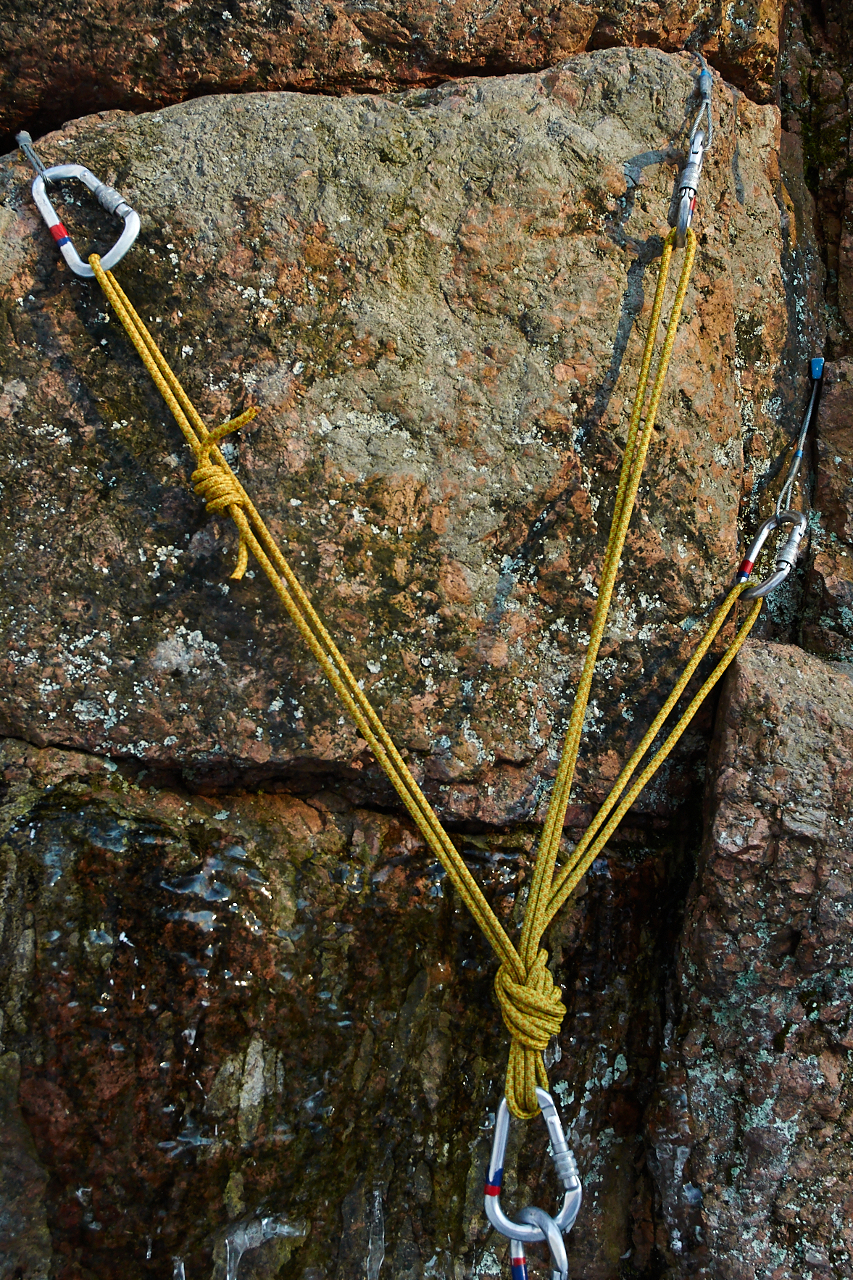
\includegraphics[width=\textwidth]{cordelette3}
            \captionof{figure}{Станция с фиксированным центральным узлом на трёх точках.}\label{fig:cordelette3}
        \end{minipage}
    \end{figure}
    
    Станция с фиксированным центральным узлом на двух точках получается натягиванием петли в направлении ожидаемой нагрузки и завязыванием узла
    (восьмёрка или проводник) для получения независимых ветвей
    (рис.~\ref{fig:cordelette2}). Станция с фиксированным центральным узлом на трёх точках делается аналогично (рис.~\ref{fig:cordelette3}).
    Для того чтобы узел легче было развязать после нагружения станции,
    в узел вставляют карабин (не нарушая целостности его структуры). Получившуюся петлю можно использовать в качестве центрального пункта станции.
    
    Нагрузка в станции с фиксированным центральным узлом распределяется равномерно между точками только если она направлена определённым образом,
    поэтому очень важна правильная настройка положения центрального узла. Если направление нагрузки меняется, то одна или несколько ветвей станции оказываются ненатянутыми и вся нагрузка приходится
    только на одну точку. Силы в станции также распределяются неравномерно если длины плеч станции с фиксированным центральным узлом не равны.
    Например, такое происходит, если все точки станции находятся в одной вертикальной щели.
    В такой конфигурации при рывке большая часть нагрузки придётся на короткую ветвь.
    
    Большим плюсом станции с фиксированным центральным узлом является отсутствие проседания при отказе одной из точек. Кроме того, станция с фиксированным центральным узлом
    быстро и просто организуется.
    
    % I do not really need this pic, right?
    %\begin{figure}
    %    \centering
    %    \includegraphics[width=0.45\textwidth]{knot_biner}
    %    \caption{Центральный пункт станции с фиксированным центральным узлом на двух точках с карабином в узле.}\label{fig:knot_biner}
    %\end{figure}

\section{Технические рекомендации}
    При организации станций полезно придерживаться следующих рекомендаций:
    \begin{itemize}
        \item Для точек станции рекомендуется использовать самые большие из имеющихся закладных элементов: самые большие гексы, самые большие закладки, самые большие камалоты.
        \item Рекомендуется использовать муфтованные карабины в точках станции. При отсутствии карабинов с муфтами используются пары немуфтованных карабинов, развёрнутые защёлками
                в противоположные друг другу стороны (рис.~\ref{fig:biners}).
        \begin{figure}[h]
            \centering
            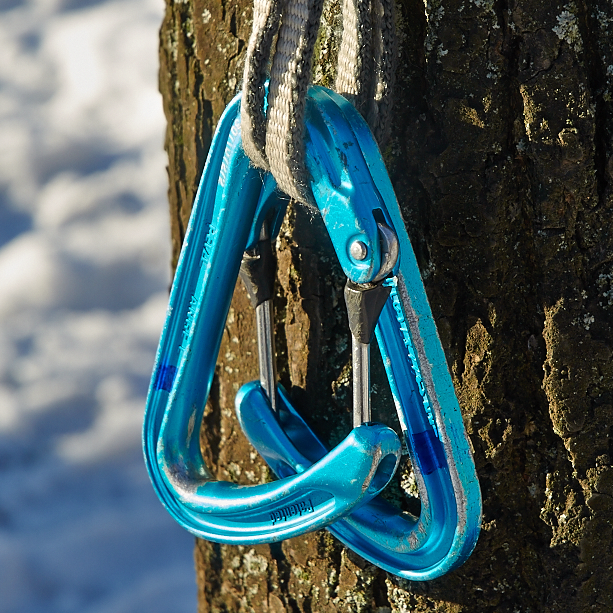
\includegraphics[width=0.45\textwidth]{biners}
            \caption{Два немуфтованных карабина, развёрнутые защёлками в разные стороны, используются для замены одного муфтованного карабина. Вщёлкиваться необходимо в оба карабина сразу.}\label{fig:biners}
        \end{figure}   
        \item Мастер-карабин -- муфтованный, замуфтовывается при организации станции первым участником и размуфтовывается только при разбирании станции последним участником.
        \item Все карабины должны быть по возможности развёрнуты <<муфтой от скалы>>.
        \item Для блокировки точек в многоточечных станциях можно использовать:
            \begin{itemize}
                \item сшитые петли из стропы из нейлона или дайнимы/спектры;
                \item петли из нейлоновой стропы связанные ленточным узлом (встречный проводник);
                \item нейлоновый репшнур 7мм связанный узлом грейпвайн;
                \item репшнур из высокопрочного материала (кевлар, дайнима/спектра и т.п.) связанный узлом грейпвайн в три оборота;
                \item основную верёвку.
            \end{itemize}
        \item Для удлинения петель рекомендуется использовать карабины, вместо пропускания петли в петлю или узла удавка.
        \item Сшивка/узел в петле не должны попадать в узлы станции и карабины и не должны мешать компенсации в станциях с динамическим распределением нагрузки.
        \item Угол между ветвями станции не должен превышать $90^o$.
    \end{itemize}
    
\nocite{*}
\bibliographystyle{plain}
\bibliography{anchors}
\end{document}
